\acresetall
\chapter{Artificial Intelligence}\label{ch:ml_intro}

\section{Overview}
\emph{Intelligence} as a concept has been a topic of exhausting research in fields such as neurology, philosophy, neuroscience, neurobiology, datascience, among others. The Oxford dictionary defines intelligence as \emph{"the ability to acquire and apply knowledge and skills"} \cite{Oxforda}. The first part of this definition applies to what is known as "learning", which is according to the accepted definition of the term as well \cite{Oxford}, and that supports, from the etymology, the importance of the process of learning on intelligence.\\

Jeff Hawkins, a dedicated neuroscientist and author, has approached the subject from the engineering and medical flanks, analysing the structure of the brain and having the perspective of the possibilities of replicating artificially the most sophisticated type of intelligence found on Earth: the human. In his book \emph{On Intelligence} \cite{HawkinsJeff2004}, he captures his findings after inspecting the brain cortex and making a parallel between humans and machines. According to Jeff, \emph{"it is the ability to make predictions about the future that is the crux of intelligence"}, and these predictions are based on the experiences from which the intelligent being has learnt, making decisions that lead it to the best possible known result. In order to create artificially a so-called \emph{intelligent agent}, scientist have put extensive effort first on trying to replicate the known intelligence \cite{Brooks1991}\cite{Reed2007}\cite{Hawkins}, taking the approach of generating a machine that is human-like and that behaves like one, being able to observe its surroundings, learn from stimulus that come from the real world, adapt to changes in those surroundings, plan accordingly to foreseeable process (therefore, make predictions), make decisions and act appropriately. These are the characteristics that Mitola \cite{Mitola1999} described in the cognition cycle for \ac{CR}, which can be applied to any intelligent agent and, consequently, motivate the further research of \ac{AI}.\\

\ac{AI}, however, encircles a variety of disciplines that are in themselves a complete course of research, as it can be seen in Fig~\ref{fig:ai}. This work focuses only in the top branch: machine learning. However, given the slight differences regarding implementation, a separate section will be dedicated solely to deep learning.

\begin{figure}[htb]
    \centering
      \includestandalone[width=\textwidth]{figures/ai_tree}
      \caption{Artificial Intelligence}
      \label{fig:ai}
\end{figure}

\section{Machine Learning}
\ac{ML} encloses the process of taking a data set that represents any phenomena and learning from it. Any type of being that is capable of learning from previous experiences is showing a kind of intelligence, as it interiorizes the stimulus/data and reacts accordingly when it presents itself again. The vast majority of living beings have this capacity, being the humans who have the lead on its effectiveness. Identifying objects, speaking languages, and reacting to any sensorial stimulus is a result of a successful learning process. \\

Generally speaking, learning from data is done when no there is no analytic solution to an encountered situation, but there is enough data to adapt to the it, generating an empirical solution to a problem that cannot be mathematically a-priori described, but that follows a specific pattern\cite{Yaser}. Just as humans do, the idea of machine learning is to generate intelligent agents computationally - teach computers to learn. The idea is as follows: a machine learning algorithm is given a set of data from which it can extract specific information that tells it the specifics about the data. With enough information, the computer is able to make predictions about other data in a different point of time if this data presents the same characteristics.

Although there is no specific mathematic representation of the specific problem to solve, many \ac{ML} algorithms relay heavily on mathematic definitions and optimization theory. Further information regarding \ac{ML} algorithms can be found in section~\ref{ch:ml_algs}. Yet is this versatility provided by the fact of not needing to pin down the specific analytic description of the problem which has impulsed this methodology into several fields of knowledge, being nowadays applied to solve problems such as financial forecasting\cite{Bose2001}, medical diagnosis\cite{Kononenko2001}, entertainment\cite{Bennett2007} and communications systems (such as this thesis), among others. Examples of everyday problems that are suitable for \ac{ML} implementation are:

\begin{itemize}
    \item Ranking links and clicks for a better web search engine and advertisements.
    \item Custom user recommendations based on purchases/rents/views.
    \item Prediction of markets and stock exchange.
    \item Dating sites with reevaluation of algorithms based on successful matches.
    \item Financial fraud detection.
    \item Supply chain optimization
    \item Biotechnology research acceleration by sequencing and screening of DNA and protein/compound structures.
    \item National security based on enormous surveillance data.
\end{itemize}

\subsection{The learning problem}
Learning from data is definitely a hot topic, which can be seen from the increasing amount of research and application that has been handed over this theory and methodology. Additionally, it is noticeable how the term has been capturing the mainstream interest and is somewhat heard-of, as it can be seen in the Fig.~\ref{fig:ml_trend}, where this trend over the past few years is clear. At this point, it is preeminent to clarify what is the purpose of \ac{ML}, and when it plays an important role. Although \ac{ML} has shown to perform outstandingly into solving many problems, it is not intended to move aside the many and well designed analytic solutions for many of the scientific existing problems, but to come in handy when that analytic solution does not describe completely the problem or does not exist. In his book \cite{Yaser}, Prof. Yaser nicely states that although many problems can be solved effectively using a learning approach or an analytic approach, the point of learning is not to compare itself and overcome the performance over the mathematical description of existing problems, but to be a complementary tool for scientist in their eagerness to solve complex problems without being stuck when facing the lack of a complete description of it.

\begin{figure}[htb]
    \centering
      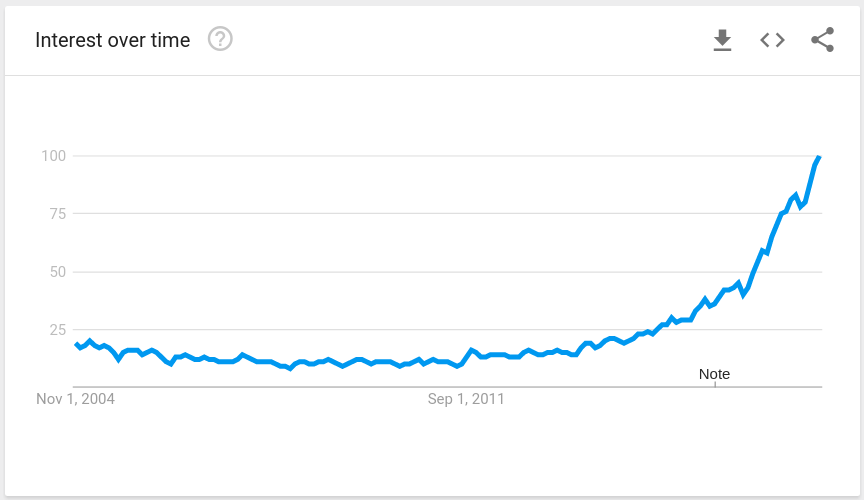
\includegraphics[width=0.6\textwidth]{figures/ml_trend.png}
      \caption{'Machine learning' Google search trend \cite{GoogleInc.2017}}
      \label{fig:ml_trend}
\end{figure}

The learning problem is summarized in the Fig~\ref{fig:learning_problem}. The learning algorithm  \( \mathcal{A} \) receives data of any form, and its solely purpose is to identify mechanisms that describe that dataset  \( \mathcal{D} \) closely. This dataset is defined as input-output samples for the supervised learning, input-weights samples for reinforcement learning and only inputs for the unsupervised learning. Further information regarding supervised, reinforcement and unsupervised learning can be found in section~\ref{ch:learning_types}. For the sake of the explanation, lets take the supervised learning case, where the dataset  \( \mathcal{D} \) includes samples of the form \( (\mathbf{x}_1, y_1),\cdots , (\mathbf{x}_N, y_N) \), where \(x\) is the input that belongs to the input space \( \mathcal{X} \), \(y\) is the corresponding output such that \(y_n = f(x_n)\), and belongs to the output space \( \mathcal{Y}\). Now, the learning algorithm \( \mathcal{A} \) needs to find that function \(f(x)\). For this, it counts with an hypothesis set \( \mathcal{H} \), which are the mathematical representations that the algorithm uses as tools to accomplish his purpose. From \( \mathcal{H} \) the algorithm takes one hypothesis \( g:\mathcal{ X \rightarrow Y} \) that approximates \(f\). After a \(g\) has been selected, the process estimates how alike the outputs from \(g(x)\) are to \(f(x)\), and feedbacks an error measure \(E(g,f)\). This process is repeated iteratively until an hypothesis produces an acceptable minimum error. \\

\begin{figure}[htb]
    \centering
      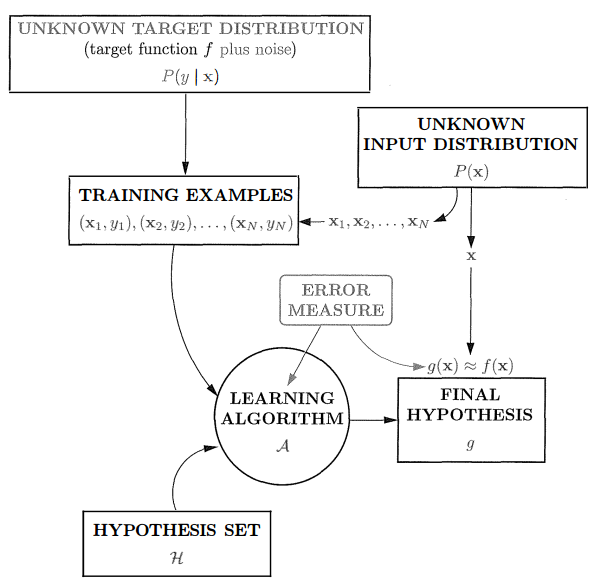
\includegraphics[width=0.6\textwidth]{figures/learning_problem.png}
      \caption{The learning problem \cite{Yaser}}
      \label{fig:learning_problem}
\end{figure}

Now, it is imperative to determine quantitatively what exactly \emph{acceptable} entitles. Different applications can have different tolerances to error, and this affects directly the hypothesis \( \mathcal{g}\) that is chosen at the end of the learning process. This means that this is an end-user parameter that has to be set as a requirement for the whole system.

After taking many different samples from \( \mathcal{X} \), and reducing the error, we should take into account the samples that \emph{we did not take}, meaning the samples that are not in our input set, and that probably behave similar to the \( \mathcal{X} \) set - i.e. we should be able to identify similar samples in order to be able to predict. Therefore, a probability distribution is added to both the input samples and the final hypothesis in order to infer from \( \mathcal{D} \) the behaviour of samples that are not in \( \mathcal{D} \). Let us assume a binary classification problem, where \( \mathcal{D} \) contains two classes A and B in a possibly infinite number of them. From a random sample pick the probability that the input sample is of the A type will be denoted as \(\mu\) and, consequently, the probability that the input sample is of the B type is 1 - \(\mu\). The value of \(\mu\) is unknown and will continue to be unknown in the process. From a random pick of N samples from \( \mathcal{D} \), there is a proportion of \(\nu\) samples of the A type, and we intend to determine how \(\nu\) relates to \(\mu\). In statistical jargon, we want to determine how our sample relates to the whole population. \\

From any point of view, the larger the sample that contributes to \(\nu\), the closer the relation it has with \(\mu\), but this relation can be quantified using the \emph{Hoeffding Inequality} \cite{Hoeffding1963}, which states that for any sample size \(N\),

\[\mathbb{P}[|\nu -\mu|>\epsilon ]\leq 2e^{-2\epsilon^{2}N} \quad \text{for any}\quad \epsilon>0\]

Where \(\mathbb{P}[\cdot]\) denotes the probability with respect to the chosen sample, and \(\epsilon\) can be any positive value chosen by the data scientist, and represents the tolerance of error. This inequality says, simply put, that as the sample size \(N\) grows, it is \emph{exponentially unlikely} that the realization \(\nu\) deviates from \(\mu\) by more than the tolerance \(\epsilon\). It can be clearly seen that the only the size of the sample \(N\) affects this bound. Consequently, to achieve a small tolerance \(\epsilon\), a large \(N\) has to be used.\\

Additionally, it is important to take into account the intrinsic noise of the systems, which can come from the nature of the input samples, i.e. the samples are not product of a deterministic system, or are immersed into some stochastic variation that can be modeled by noise, and that implies that by having the same input into the system \emph{it is probable} get a different output. This entails a change in the labels of the model. That is, instead of having \(y = f(x)\), we take \(y\) as a random variable resulting from a probability distribution \(P(y|x)\). Accordingly, the input data points are therefore generated by the joint distribution \(P(x,y) = P(x)P(y|x)\). With this description of the model, our target function (what \(\mathcal{A}\) wants to learn) becomes \(P(y|x)\), while \(P(x)\) quantifies the importance of the input \(x\) in our learning accuracy.

\subsection{Types of learning}\label{ch:learning_types}

There are three types of learning: supervised-, unsupervised-, and reinforcement learning. Each of them  has specific characteristics, which are explained in the following subsections.

\subsubsection{Supervised Learning}
Is the type of learning where, in addition to the input dataset, the explicit correct outputs for those given inputs are given to the \ac{ML} algorithm for training. There are two types of supervised learning:
\begin{itemize}
    \item \textbf{Classification:} its main goal is to predict a \emph{class label} from a determined set of choices. If the number of choices is two, the model corresponds to a \emph{binary classification}. As it has only two options, it is suitable for problems whose expected answer is of the form "yes/no", "present/not present", "valid/invalid". For a greater number of classes the model corresponds to a \emph{multiclass classification}. Examples of classification are:
        \begin{itemize}
            \item Determining whether an email is spam or not constitutes a binary classification problem.
            \item Identifying the zipcode from handwritten digits on an envelope is a multiclass classification problem.
            \item Determine whether a tumor is benign based on size and shape data constitutes a binary classification problem
        \end{itemize}
    \item \textbf{Regression:} its purpose is to predict a continuous behaviour, such as a trend, or a floating-number, and it is this continuity what sets it apart from the classification models. Examples of regression are:
        \begin{itemize}
            \item Predict the value of the stock market
            \item Determine the expected amount of crops yield from a plantation based on data such as previous yields, weather history, etc.
        \end{itemize}
\end{itemize}

\subsubsection{Unsupervised Learning}
Unlike supervised learning, here the algorithms are feed with data but not with the expected outputs, which make this type of learning suitable for solving problems to which the output is unknown. The model is then in charge of extracting knowledge from the input data all by itself, without no further instructions. There are mainly two types of unsupervised learning that can be found in the literature \cite{Andreas}, which are the \emph{unsupervised transformations} and \emph{clustering}.

\begin{itemize}
    \item \textbf{Unsupervised transformations:} are models in charge of creating new representations of the input data, so that it becomes easier to understand and/or to use than the original data. This functionality is used, for example, to reduce the dimensionality of data that consists of several features. In such situation, the model transforms the data into a representation that summarizes the input with fewer features. Another important use of this type of models is finding the overall representation of the input data, such as the topic of a full text, or the sentiment in a short comment.
    \item \textbf{Clustering:} this kind of models group the data into determinate groups that share similar characteristics. This is used, for example, to generate suggestions based on previous purchases/views, or to group pictures from a directory with several images to the ones that contain certain people (and suggest tagging the names on them).
\end{itemize}

As the models do not know beforehand what type of information they are intended to learn, one of the tasks of the data scientist is to assess that the model is indeed learning something useful. This creates the opportunity for this sort of models to be used for the same data scientist to help them identify certain characteristics of the data that were not obvious for the \emph{human-eye}, and certainly get a different perspective of the data from the \ac{ML} model point-of-view.

\subsubsection{Reinforcement Learning}
This type of learning has a different approach to the previous two descriptions. Just like unsupervised learning, the model does not receive the expected outputs for the inputs it is given but, in contrast, it receives some output \emph{possible} output along with a weight that states how good of an output it is. The idea behind this is that the model is then penalized when it provides a solution that is not according with the possible output, and is rewarded when it is. Then, the model uses this penalizations and rewards to adjust the type of outputs it generates, and so it eventually learns the correct behaviour for the situations it has been immerse into. This type of learning is similar to the way humans learn, in ways such as being penalized with pain when taking a sip of very hot coffee, or rewarded with winning a game of chess.\\

In that same manner, reinforcement learning comes in handy in teaching an intelligent agent how to play a game, where it is presented to a plethora of options (which makes it difficult to be modeled as a supervised learning problem) and has to choose the one that brings it near to victory. The most recent example is AlphaGo \cite{Fu2017}, an intelligent agent capable of winning the world Champion on a Go game. A similar approach has been followed by IBM's with the Deep Blue chess-playing machine \cite{Hsu1999}.

\subsection{Training Models}

\subsection{Testing Models}
\subsection{Model Evaluation}
\subsubsection{Overfitting}
\subsubsection{Underfitting}
\subsection{Data preprocessing}
The main requirement of \ac{ML} is that data is the main requirement. In the same way, it is necessary to ensure that the data is valid and that information can be extracted from it.
\subsubsection{Data transformation and scaling}
\subsection{Feature Engineering}

UNSUPERVISED LEARNING CAN BE USED FOR FEAUTURE EXTRACTION andreas page 154 (PCA)

\subsection{Machine Learning algorithms}\label{ch:ml_algs}
\subsubsection{K-nearest Neighbors}
\subsubsection{Support Vector Machines}
\subsubsection{Binary trees}

\section{Deep Learning}
\subsection{Neural Networks}
\subsection{Convolutional Neural Networks}
\section{Optimization of Cost Functions}

